\documentclass[usegeometry=true]{scrartcl}
\usepackage[ngerman]{babel}
\usepackage[T1]{fontenc}
\usepackage{lmodern}
\usepackage[utf8]{inputenc}
\usepackage{hyperref}
\usepackage{amssymb}
% Dimensionen bitte nicht ändern. 
\usepackage[left=2cm, right=2cm, top=2cm, bottom=2cm, bindingoffset=1cm, includeheadfoot]{geometry}
%Zeilenabstand bitte nicht ändern
\usepackage[onehalfspacing]{setspace}
\usepackage{graphicx}
\usepackage{float}
\usepackage{prettyref}
\usepackage[backend=biber,style=numeric,]{biblatex}\addbibresource{literatur.bib}

\begin{document}
\pagenumbering{gobble}
\subject{Projektbericht zum Modul Information Retrieval und Visualisierung Sommersemester 2022}
\title{Analyse des Kaufverhaltens in Supermärkten}
%\subtitle{Untertitel}% optional
\author{Konstantin Wohllaub}% obligatorisch
%\date{10.9.2022}
\dedication{\normalsize\vfill\hrule\vspace{10pt}
	Link zum GitLab-Repository:\\
	\url{https://gitlab.informatik.uni-halle.de/amhvy/supermaket-sales}\\
	\vspace{10pt}
	Link zur öffentlich zugänglichen Webseite (GitHub Pages):\\
	\url{--}}

\maketitle% verwendet die zuvor gemachte Angaben zur Gestaltung eines Titels
\newpage
\tableofcontents
\newpage
\pagenumbering{arabic}
\section{Einleitung}
Seit jeher gibt es zwischen Unternehmen in der Wirtschaft einen Kampf um steigende Gewinne und zahlende Kunden.
In Zuge dessen wird von Seiten der Unternehmensleitungen versucht, einen Vorteil gegenüber ihren Konkurrenten zu erreichen.
Dieser Vorteil wird vorallem, durch die in den letzten Jahren sehr beliebt gewordene Datenanalyse erreicht.
Bis vor ein paar Jahren war die Verarbeitung von solch großen Datenmengen undenkbar,
jedoch machte der enorme Anstieg von Speicher- und Rechenkapazität sowie Fortschritte in der Softwareentwicklung dies in den letzten Jahren möglich.\cite[1]{emrouznejad2016big}
Da der einfache Besitz dieser großen Datenmengen den Unternehmensführungen von nicht all zu großen Nutzen ist, müssen die Daten noch aufbereitet, analysiert und interpretiert werden.\cite[1]{Tien2013}
Dabei wird versucht bestimmte Muster oder Verhaltensweisen zu finden, die letztendlich zu einem Wettbewerbsvorteil gegenüber anderen Marktteilnehmer führen können.

\noindent Die Einzelhandels-Branche gehört zu den Branchen, die mit am meisten Daten generiert.
Jeden Tag strömen Millionen von Menschen in die Einkaufsläden, um Produkte des alltäglichen Bedarfs zu besorgen.
Da durch jeden einzelnen Kunden und jedes einzelne gekaufte Produkt wertvolle Daten generiert werden, hat die Einzelhandels-Branche den Vorteil auf eine sehr ausführliche
Datenansammlung zurückgreifen zu können.
Aus diesem Grund hat unter anderem Walmart, eines der größten Unternehmen auf der Welt, im Jahr 2015 angekündigt, die größte Private Data Cloud der Welt
zu erstellen.\cite[5]{marr2016big}
Zusätzlich zu der sehr hohen Datendichte, ist die Einzelhandels-Branche auch eine der kompetetivsten Branchen, da es in kaum einer anderen Branche
so viele gleichwertige Akteure am Markt gibt, die miteinander konkurrieren.\cite{Grewal2010}
Aus diesem Grund sind es vorallem Unternehmen, die Supermärkte betreiben, die auf die Datenanalyse zurückgreifen müssen, um sich von der Konkurrenz abzuheben.
Auf Grundlage dessen versuchen die Supermärkte dann ihr Angebot so zu gestalten, dass der Nutzen der Kunden maximiert wird, sodass diese gewillt sind, diesen Einkaufsladen den anderen vorzuziehen.\cite[6]{marr2016big}
Zuvor müsssen sich die Supermärkte jedoch Fragestellungen überlegen, um überhaupt zu wissen, wonach gesucht werden soll.

\noindent Genau hier an diesem Punkt soll die Projektarbeit anknüpfen und aus der Sicht einer Supermarktleitung, sich möglich ergebende Fragen, zu beantworten.

\begin{itemize}
	\item Sind bestimmte Muster in den Daten zu erkennen, die auf Abhängigkeiten zwischen Kaufattributen deuten ?
	\item Welche Kunden sind am profitabelsten ?
	\item Welche Produkte sind am profitabelsten ?
	\item Gibt es Ausreißer und falls ja, warum ?
\end{itemize}

\subsection{Anwendungshintergrund}
Bei dem Kauf eines Produkt in einem Supermarkt werden, wie in der Einleitung bereits beschrieben, viele Informationen generiert. Unteranderem kann festgestellt werden,
welches Geschlecht der Kunde hat, was er für Produkte einkauft, welchem Segment diese Produkte zugehörig sind, wie viele Produkte von einer Sorte gekauft werden,
wie viel er dafür insgesamt bezahlt und vieles mehr. Im optimalen Fall sammeln Supermärkte diese Daten, um sie in einem Datensatz zu speichern.
Der Datensatz der im Zuge dieser Arbeit analysiert und visualisiert wurde, ist das Ergebnis einer solchen Datensammlung. Nun kann durch spezielle
Informationsvisualisierungstools dieser Datensatz ausgewertet werden, um Rückschlüsse oder Vorhersagen bzgl. des Kundenverhaltens machen zu können.
Da es aber oftmals schwer ist Muster in der Gesamhtheit der Kundendaten zu erkennen, kann es, speziell für Supermärkte, sinnvoll sein die Daten nach gewissen Eigenschaften zu
filtern. Dies ermöglicht es zum Beispiel Information bzgl. des Kaufverhaltens von Männern und Frauen sowie von einkommenstarken und einkommenschwachen Kunden zu bekommen.


\subsection{Zielgruppen}
Die Zielgruppe dieser Arbeit besteht in erster Linie aus den Unternehmensführungen von Supermärkten, die sich in Ländern mit ähnlichen demographischen und kuluterellen
Gegebenheiten befinden, wie die Supermärkte von denen die Daten gesammelt wurden. Die Unternehmensleitungen können aus der Arbeit wichtige Informationen hinsichtlich ihres
operativen Geschäfts ziehen undihr bereits vorhandenes Wissen damit erweitern. Zudem können die Ergebnisse dieser Arbeit auch für die Marketing-Abteilungen der Unternehmen
interessant sein, da sie durch die zusätzlich Informationen über ihre Kunden, die Werbekampagnen besser auf die Bedürfnisse der Kunden abstimmen können.

\noindent Auf der anderen Seite können auch die Kunden selbst, von den Visualisierungen dieser Arbeit profitieren. Dadruch, dass nicht nur das Kundenverhalten im Fokus steht,
sondern auch Attribute wie z.B. Kundenzufriedenheit oder Verkaufspreis, können die Kunden einsehen, wo der Service und die Preise am optimalsten für sie selbst sind.

\subsection{Überblick und Beiträge}
In dem verwendeten Datensatz sind alle Einkäufe aufgelistet, die es in einem Zeitraum von drei Monaten in den drei myanmarnesischen Städten Yangon, Naypyitaw, Mandalay gab.
Dabei wurden die drei Zweigstellen in den drei Städten, der nicht namentlich genannten Supermarktkette, betrachtet. In dem Datensatz wurden produkt- und kundenspezifische
Daten quantitativer und qualitativer Natur erfasst. Bei den produktspezifischen Daten handelt es sich nicht um einen kompletten Warenkorb, sondern
um einzelne Produkte und deren gekauften Anzahl.

\noindent Die Umsetzung der Visualisierung erfolgt durch genau drei Techniken: Scatterplot, Parallele Koordinaten und eine Pixelorientierte Darstellung mithilfe der Recursive Pattern
Technik. Auf die einzelnen Visualisierungstechniken wird im späteren Verlauf der Arbeit noch genauer eingegangen.

\noindent Der Beitrag dieser Arbeit setzt sich aus der Visualisierung des zugrunde gelegten Datensatzes und denen daraus resultierenden Informationen zusammen. Der Lesende erhält
dadruch ein Einblick in das Kunden- und Kaufverhalten im Bezug auf Supermärkte. Diesen Einblick und die damit erlangten Informationen können dann genutzt werden, um Sie für
weiterführende Forschungszwecke ökonomischer Natur einzusetzen.

\section{Daten}
Wie oben bereits angedeutet, ist der in der Arbeit verwendete Datensatz eine Sammlung von Kunden- und Kaufdaten aus drei verschiedenen Zweigstellen eines Supermarkt
Unternehmens in Myanmar. Die verschiedenen Zweigstellen befinden sich in den Städten Yangon, Naypyitaw und Mandalay. Mandalay und Naypyitaw haben knapp über 1 Million Einwohner,
Yangon sogar über 5 Millionen Einwohner. Jede Zeile des Datensatzes besteht aus einer Computergenerierten Rechnungsnummer, zur eindeutigen Identifikation des Kaufes, sowie dem
Produkt, dass gekauft wurde. Hinzu kommen Daten über den Kunden, wie Geschlecht, Kundenstatus, Einkommen des Kunden und Bewertung des Kaufes sowie folgende Daten über das Produkt:
Verkaufspreis, Produktlinie, Kosten des Produkts für den Supermarkt, Anzahl gekaufter Produkte, Gesamtausgaben(Verkaufspreis*Anzahl gekaufter Produkte), Steuer,
Preis inklusive Steuer und die prozentuale Gewinnspanne.
Dieser Umfang an Daten je getätigten Kauf stellt sicher, dass eine umfassende Analyse, bezüglich des Kaufverhaltens der Kunden sowie der Verkaufsperformance des Supermarkts,
möglich ist. Alle in der Einleitung aufgestellten Fragen können somit beantwortet werden. Durch Daten auf Kunden- und Produktseite ist es zudem möglich die verschiedenen
Zielgruppen, welche bereits definiert wurden, mit den geeigneten Informationen zu bedienen. Aus diesem Grund war es nicht nötig, den Datensatz mit zusätzlichen Daten zu erweitern.

\subsection{Technische Bereitstellung der Daten}
Der Datensatz ist auf der Website von kaggle unter den Link: \url{https://bit.ly/3eco5mX} zu finden. Dieser ist dort als csv-Datei frei verfügbar. Die csv-Datei wurde im
folgenden repository: \url{https://github.com/Konwoh/Information-Retrieveal} auf GitHub gespeichert. Anschließend wurde die raw-Version der csv-Datei durch eine HTTP-Anfrage
in das Programm geladen, um dort weiterverarbeitet zu werden. Der Datensatz wurde auch zusätzlich in dem finalen repository auf GitLab zur Überprüfung bereitgestellt.

\subsection{Datenvorverarbeitung}
Da der Datensatz in einer einzigen csv-Datei bereits vorlag, ersparte dies etliche Schritte der Datenvorverarbeitung. Einzig allein die Datumsspalte wurde vor dem Einladen
in das Programm mithilfe der Python Bibliothek Pandas verändert. Dabei wurde das Datum, dass in der csv-Datei als String in der Form YYYY/MM/DD gespeichert war, in ein
Datumobjekt der Form YYYY-MM-DD geändert. Dieser Schritt war notwendig, da das ELM-Paket Date (\url{https://package.elm-lang.org/packages/justinmimbs/date/latest/Date}),
nur Datumsangaben in der Form YYYY-MM-DD akzeptiert. Der beschriebene Schritt war auch gleichzeitig der einzige Schritt der nicht in ELM programmiert wurde.

\noindent Da die csv-Datei nun im ELM-Programm zur Verfügung steht, mussten nun Datentypen definiert werden, in denen die Zeileninhalte des Datensatzes überschrieben werden.
Hierfür gab es den primären Datentyp Sale und mehrere Unterdatentypen wie z.B. das Geschlecht oder die Produktlinie. Nichtsdestotrotz waren die Unterdatentypen trotzdem ein
Bestandteil des primären Datentyps Sale. Damit die Überschreibung der Daten von der csv-Datei in die gewünschten Datentypen erfolgreich stattfindet, musste ein Decoder
geschrieben werden. Die salesDecoder-Funktion, die Funktionalitäten des Elm-Pakets elm-csv (\url{https://package.elm-lang.org/packages/BrianHicks/elm-csv/latest/}) benutzt, war
dafür verantwortlich. Mit Anwenden dieser Funktion auf den geladenen Datensatz, war die Datenvorverarbeitung nun abgeschlossen.

\section{Visualisierungen}
\subsection{Analyse der Anwendungsaufgaben}
Die Anwendungsaufgaben der Anwender und Anwenderinnen ergeben sich zunächst aus der bloßen Betrachtung und den damit verbundenen Verstehen der einzelnen Visualisierungstechniken.
Danach sollen durch die verfügbaren Variationen, die von den Visualisierungstools zur Verfügung gestellt werden, genau die Attribute betrachtet werden, die für den Anwender
interessant und wichtig erscheinen. Dadruch sollte es den Betrachter möglich sein, die in der Einleitung aufgestellten Fragestellungen zu beantworten. Dabei ist auch wichitg zu
erwähnen, dass die betrachtete Stichprobe von den Betrachter eingegrenzt werden kann. Dies kann z.B. nach Geschlecht oder Art der Zahlung erfolgen, was sich ebenfalls positiv
auf die Beanwortung der Fragestellungen auswirken sollte.

\noindent Die Visualisierungen zeigen den Betrachtern bestimmte Zusammenhänge zwischen den gewählten Attributen auf, was unter anderem Rückschlüsse auf Korrelation
und Beziehung der einzelnen Attribute untereinander ermöglicht. Da durch die Visualisierung die Daten in einen bestimmten Kontext gerückt werden, wird es dem Betrachter somit
ermöglicht, die Daten besser in der realen Welt einzuordnen. Die daraus resultierenden und besser zu greifenden Vorstellungen können den Anwender schließlich bei der Lösung der
Aufgaben ebenfalls behilflich sein.

\noindent Die eben beschriebenen Vorstellungen oder mentalen Modelle sind sehr wichtig für die Beantwortung der Aufgaben, da z.B. auf die Frage wer der profitabelste Kunde sei,
keine einfache Antwort zu geben sei ohne alle Zusammenhänge sowie Beziehungen der Attribute zueinander graphisch darzustellen. So gibt es zum Beispiel Kunden, die zwar viele
Produkt kaufen, aber dafür nur die billligsten. Andererseits gibt es Kunden, die nur wenige Produkte kaufen, die dafür aber sehr teuer sind. Mentale Modelle lassen sich jedoch
durch diese textlich beschriebenen Vebrindungen und Abhängigkeiten nur sehr schwer bilden, weshalb es umso wichtiger ist, dies in der visuellen Form dazustellen.

\subsection{Anforderungen an die Visualisierungen}\label{Anforderung}
Laut Schumann und Müller sollen Visualisierungen expressiv, effektiv und angemessen sein. \cite[9]{schumann2013visualisierung} Genau diese grundlegenden Anforderungen bestehen
auch bei der Visualisierung der hier verwendeten Daten.

\noindent Um die zu Beginn aufgestellten Fragestellungen zu beantworten ist auch die Existenz von spezifischeren Anforderungen notwendig. Als erstes wäre da eine Filterung der
Daten nach den gewünschten Kriterien zu nennen. Denn um eine Antwort auf die Frage: "Wer sind die profitabelsten Kunden?" zu finden, muss erstmal eine Filterung nach Kundengruppen
möglich sein. Das gleiche gilt auch für die Frage bezüglich der Produkte und der anschließenden FIlterung nach Produktgruppen. Die Filterung nach den gewünschten Kriterien
sollte der Anwender dann auch selbst durch Buttons oder Textfelder vollziehen können.

\noindent Desweiteren muss eine Visualisierungstechnik auch ermöglichen, Zusammenhänge zwischen Attributen in den Kontext des gesamten Datensatzes zu setzen. Wenn in einer Frage,
die Profitabilität behandelt wird, können z.B. mehrere Attribute für die Profitabilität stehen und nicht nur der Verkaufspreis eines Produkts, sondern auch die
Anzahl, wie oft es gekauft wurde oder die Kosten, die der Supermarkt für dieses Produkt zahlen musste. Durch den Einfluss mehrere Attribute auf die Beantwortung einer Frage, muss
es daher möglich sein, die Daten mehrdimensional darzustellen.

\noindent Als letzte Anforderung wäre noch die Identifikation von Ausreißern in den Daten zu nennen. Hier sollte es möglich sein, Daten, die sich deutlich von der Norm abheben,
auszumachen und Details zu ihnen einsehen können.

\subsection{Präsentation der Visualisierungen}
\subsubsection{Visualisierung 1: Scatterplot}\label{Visualisierung1}
Die erste gewählte Visualisierungstechnik ist ein Scatterplot oder auch Streudiagramm. Bei einem Scatterplot werden zwei numerische Attribute mittels zwei Achsen skaliert und die
jeweiligen Datenwerte einem x- sowie y-Wert zugewiesen. Diese x- und y-Werte werden dann in einem Punkt zusammengefasst und in dem Scatterplot gezeichnet. Sinn eines Scatterplot
ist es Zusammenhänge oder andere auffällige Muster zwischen numerischen Attributen festzustellen. \cite[103]{Friendly2005} Welches numerische Attribut auf welcher Achse
abgebildet wird ist im Zuge dieses Projekts vom Anwender frei wählbar. Zudem werden nur die Datenpunkte dargestellt, die zuvor vom Anwender nach gewünschten nominalen
Attributen herausgefiltert wurden. Die Filterung der Daten kann durch zwei unterschiedliche Filter angewendet werde. Daher ist es möglich den kompletten Datensatz z.B. nach
dem Geschlecht oder der Produktgruppe zu filtern oder beide Kriterien gleichzeitig anwenden und somit nur die Dateneinträge bekommen, die dem ausgewählten Geschlecht und der
ausgewählten Produktgruppe entsprechen. Dies ermöglicht eine erweiterte Eingrenzung, der zu betrachteten Stichprobe. \\
\begin{figure} [H]
	\begin{center}
		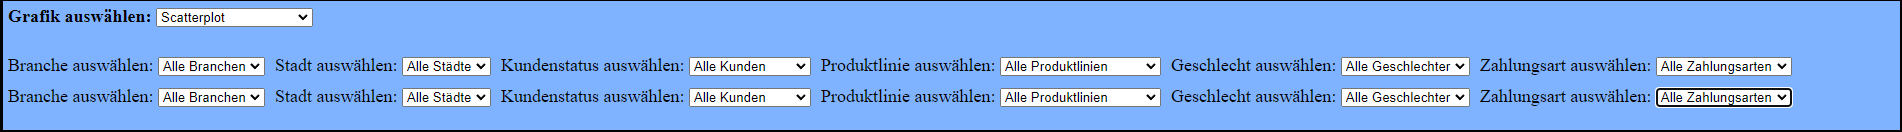
\includegraphics[width=16cm]{IMG/Filterung}
		\caption{Filterungsbuttons der Daten}
		\label{fig:Filterung}
	\end{center}
\end{figure}

\noindent Der Scatterplot erfüllt sehr gut die grundlegenden Anforderungen der Expressivität, der Effektivität und der Angemessenheit. Der Scatterplot ist expressiv, weil er
sehr intuitiv zu verstehen ist und deutlich zeigt, ob Zusammenhänge oder sonstige Muster zwischen den zwei gewählten Attributen vorherrschen. Zudem ist die eindeutige
Zuweisung der Datenpunkte zu ihren jeweiligen Reihen in dem Datensatz durch das Anzeigen einer eindeutigen Identifikationnummer, während des Hovern über dem
Datenpunkt, gewährleistet. Der Scatterplot ist effektiv, weil er ohne großen Aufwand sehr viele und nützliche Informationen darstellen kann. Und er ist angemessen, da
es eine der trivialsten Möglichkeiten ist, um zwei numerische Attribute aufeinander darzustellen. Daten-Ausreißer sind bei dieser Visualisierungstechnik ebenfalls leicht zu
identifizieren, da die Entfernung von Punktelinien oder Punktewolken sehr gut erkennbar ist.
werden.\\
\begin{figure} [H]
	\begin{center}
		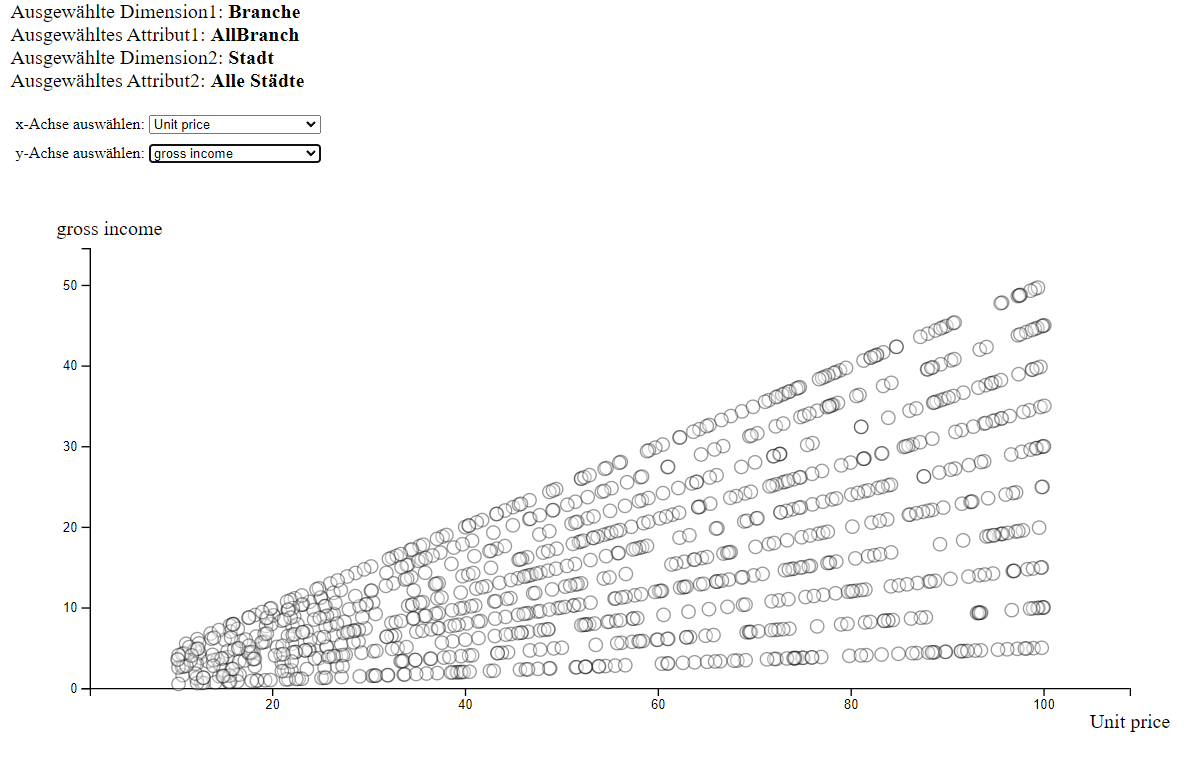
\includegraphics[width=13cm]{IMG/Scatterplot}
		\caption{Visualisierung Eins - Scatterplot}
		\label{fig:Scatterplot}
	\end{center}
\end{figure}
\noindent Die Scatterplot-Technik ist für den zu untersuchenden Datensatz perfekt geeignet, weil für die Beantwortung einiger Fragestellungen immer eine Betrachtung von
zwei Variablen in verschiedenen Kombinationen notwendig ist. Damit es möglich z.B die Beziehung von der Variable \textit{Anzahl gekaufter Produkt} mit der Variable
\textit{Bruttoeinkommen} oder die Beziehung der Variablen \textit{Rating} und \textit{Gesamtpreis} zu vergleichen. Hierbei kann der Anwender nach belieben die ihn interessierenden
Attribute miteinander kombinieren.
Des Weiteren kann durch die eindeutige Zuweisung der Datenpunkte zu ihren Datenreihen, zusätzliche Analysen bzgl.
des gewählten Datenpunktes stattfinden. Diese Analysen könnten im weitern Verlauf dazu genutzt werden, um an weitere Erkenntnisse zu gelangen.
\noindent Ebenbürtige Alternativen zum Scatterplot sind kaum verfügbar. So sagten unteranderem schon Friendly und Denis in ihrem Werk über Scatterplots:
\begin{quote}"Indeed, among all the forms of statistical
	graphics, the humble scatterplot may be considered
	the most versatile, polymorphic, and generally useful invention in the entire history of statistical graphics."\cite[103]{Friendly2005}
\end{quote}

Diese Aussage unterstreicht nochmal die Bedeutung die Scatterplots in der statistischen Analyse besitzen.
Die einzige Alternative, die in Erwägung gezogen werden kann, ist der Quantil-Quantil-Plot. Hierbei werden ebenfalls zwei numerische Attribute auf Achsen skaliert und
miteinander verglichen, allerdings beschränkt sich hier der Vergleich auf die Verteilungen der beiden Variablen. Aus diesem Grund ist diese Visualisierungstechnik nicht wirklich
für die Anwendung im Rahmen dieses Projekts geeignet, da die Verteilungen der Variablen für die Beantwortung der Problemstellungen keine Rolle spielen.

\subsubsection{Visualisierung 2: Parallele Koordinaten}\label{Visualisierung2}
Die zweite gewählte Visualisierungstechnik sind die Parallelen Koordinaten. Hierbei werden die Attribute einer Datenreihe durch einen Linienzug entlang vertikaler zueinander
paralleler Achsen dargestellt. \cite[594]{Lehmann2010} Dadurch wird die Problematik der Scatterplots, nur zwei Dimensionen anstatt multivariater Daten darstellen zu können,
behoben.\cite[1]{Wegman1990} Auf den verschiedenen Achsen können nun alle numerischen Attribute skaliert und nebeneinander angeordnet werden. Der Anwender hat zusätzlich die
Möglichkeit die verschiedenen Achsen miteinander zu tauschen, um andere mehrdimensionale Zusammenhänge betrachten zu können.
\begin{figure} [H]
	\begin{center}
		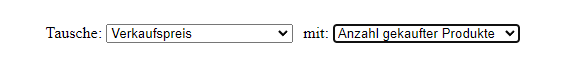
\includegraphics[width=15cm]{IMG/Achsentausch.png}
		\caption{Buttons für Achsentausch}
		\label{fig:Achsentausch}
	\end{center}
\end{figure}
\noindent Dadurch wird auch eine der zu Beginn definierten Anforderungen an die Visualisierungen, erfüllt. Bei Datensätzen, die Kunden- und Kaufverhalten beinhalten, ist es essenziell
auch die Zusammenhänge mehrerer Variablen gleichzeitig betrachten zu können. So kann es nicht nur interessant sein, die Beziehung der Variablen Bruttoeinkommen und Gesamtpreis
zu betrachten, sondern noch zusätzlich das Rating des Kaufes miteinzubeziehen.\\
Die Expressivität ist bei den parallelen Koordinaten ein bisschen niedriger einzuordnen als bei
dem Scatterplot, da für einen Beginner Parallele Koordinaten auf den ersten Blick schwieriger zu verstehen sind. Des Weiteren können Darstellungen in dieser Form schnell unübersichtlich
werden, da Linien verschiedener Datenreihen sich überschneiden können und somit unklar ist, welche Linie wohin führt. Aus diesem Grund wurden, wie im Abschnitt
\ref{Visualisierung1} bereits beschrieben, die zwei Filterungsstufen eingeführt, um die zu betrachtende Stichprobe zu verkleinern und dadruch so übersichtlich wie
möglich zu halten. \\
Die Effektivität dieser Visualisierungstechnik ist dagegen umso besser, da durch einen übersichtlichen Parallele Koordinaten-Plot viel mehr Informationen zum
Anwender transferiert werden können als es z.B. bei einem Scatterplot der Fall ist. Dieser kann, wie zu Beginn dieses Abschnitts beschrieben, sehr schnell die Zusammenhänge von
mehreren Variablen begutachten und anschließend seine Analysen vollziehen. Einzig allein die Kombinationsmöglichkeiten bezüglich der Anordnung der Achsen kann ein Problem
darstellen. Denn es ist zu beachten, dass bei k Variablen k! Achsenreihenfolgen möglich sind.\cite[594]{Lehmann2010}

\begin{figure} [H]
	\begin{center}
		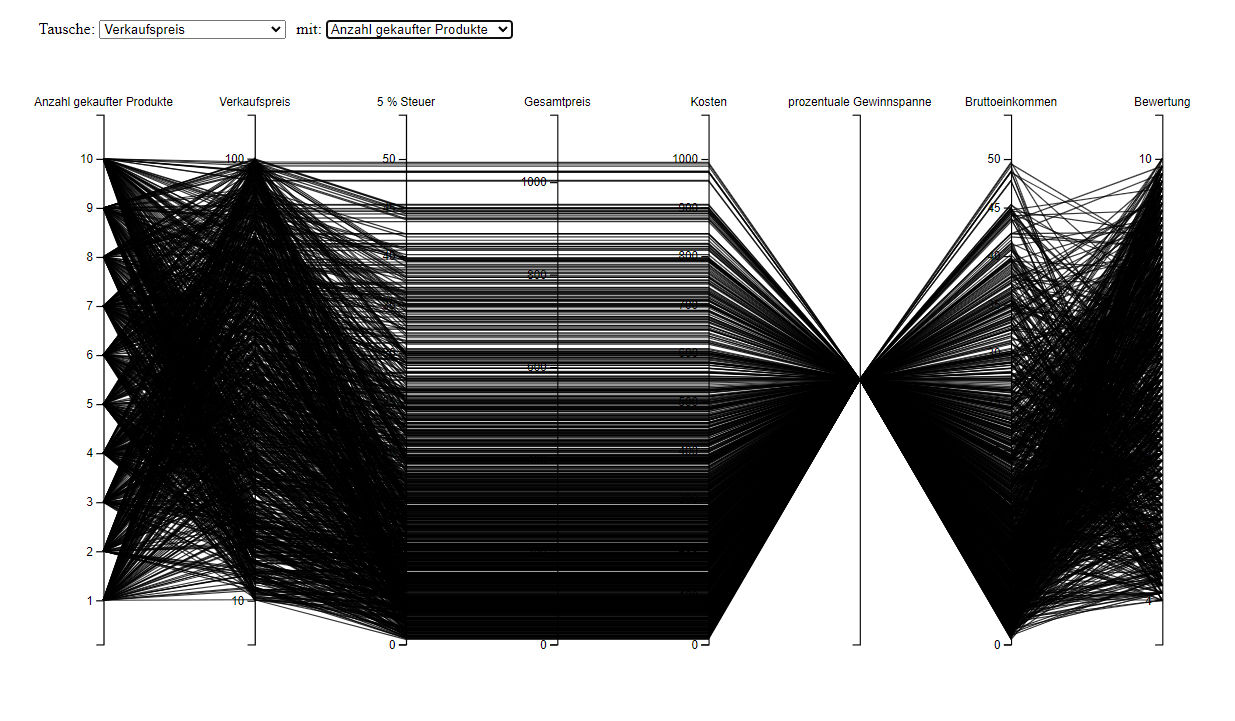
\includegraphics[width=15cm]{IMG/ParCoord}
		\caption{Visualisierung Zwei - Parallele Koordinaten}
		\label{fig:ParCoord}
	\end{center}
\end{figure}
Als Alternative zu den Parallelen Koordinaten ist die Visualisierung mittels Icon zu nennen. Hierbei wird jede Datenreihe von einen sogenannten Icon repräsentiert. Die
Attribute der Datenreihe werden durch Farbe, Form oder Ausrichtung an den Icons visualisiert. \cite[14]{a3096a239a3d49e49e8ffde9a34d754a} Durch das unterschiedliche Aussehen
der Icons kann der Anwender leicht viele Informationen extrahieren. Die bekanntesten Beispiele für Icons sind Stick Figues, Chernoff-Gesichter, Colour Icons und Glyphen.
\cite[14-16]{a3096a239a3d49e49e8ffde9a34d754a} Allerdings gestaltet es sich in manchen Fällen als äußerst schwer heraus durch die Icon-TEchnik Informationen über den gesamten
Datensatz zu erhalten, da die Visualisierung der Attribute auf den Icons, sich nur schwer unterscheiden lassen. Nur mit einer sehr detaillierten Legende kann dem Anwender
genug Hintergrundwissen zur Verfügung gestellt werden, um diese Technik sinnvoll zu nutze. Der damit verbundene Aufwand ist allerdings weit größer im Vergleich zu den parallelen
Koordinaten, weshalb sich letztendlich nicht für die Visualisierung durch Icons entschieden wurde.

\subsubsection{Visualisierung Drei - Pixelorientierte Darstellung}\label{Visualisierung3}
Die dritte gewählte Visualisierungstechnik ist die Pixelorientierte Darstellung. Bei dieser Technik werden ausgewählte Attribute durch einen farbigen Pixel dargestellt. Diese
farbigen Pixel werden anschließend durch die sogenannte Recursive Pattern Technik in eine strukturierte Anordnung gebracht, sodass dem Anwender das Lesen und Verstehen dieser
Daten einfacher gelingt. \cite[5]{Kriegel1996Visua-5711} Hierbei ist es unteranderem möglich die Pixel von links nach rechts, Zeile für Zeile anzuordnen oder auch von oben nach
unten, Spalte für Spalte.\cite[2]{485140} Im Zuge dieses Projekts wurde die Variante von links nach rechts genommen, da dies der Lesegewohnheit entspricht. \\
Diese Technik erfüllt die letzte Anforderung im Abschnitt \ref{Anforderung}. Sie stellt sicher, dass Ausreißer in den Daten sofort erkennbar sind. Dies wird durch
eine deutliche farbliche Hervorhebung gewährleistet. Für den Anwender ist zudem eine Legende über der Visualisierung eingefügt, die ihm dabei helfen, die verwendeten Farben im
Kontext des Datensatzes richtig einschätzen zu können. In diesem Projekt wurde deshalb eine Farbskala genommen, die verhältnismäßig kleine Werte kälteren Farben zuordnet und höhere
Werte wärmeren Farben.\\
\begin{figure} [H]
	\begin{center}
		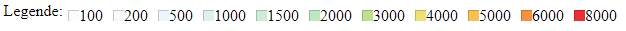
\includegraphics[width=15cm]{IMG/LegendePixel.png}
		\caption{Legende der Pixelorientierten Darstellung}
		\label{fig:LegendePixel}
	\end{center}
\end{figure}

\noindent Die Effektivität bei der Pixelorientierten Darstellung ist sehr gut, da die farblichen Pixel sehr gut mit der menschlichen Wahrnehmung synergieren und hohe Werte mit ihren
dazugehörigen warmen Farben sehr schnell ins Auge fallen. Zudem wurde für das weitere Verständnis die zu visualisierende Zeitreihe mit dem ausgewählten Attribut unter der
Visualisierung dargestellt. Somit kann der Anwender schnell die Farben in der Darstellung mit den Werten aus der Liste verknüpfen und hat zusätzlich noch das Datum, wann dieser
Wert entstanden ist.\\

\begin{figure} [H]
	\begin{center}
		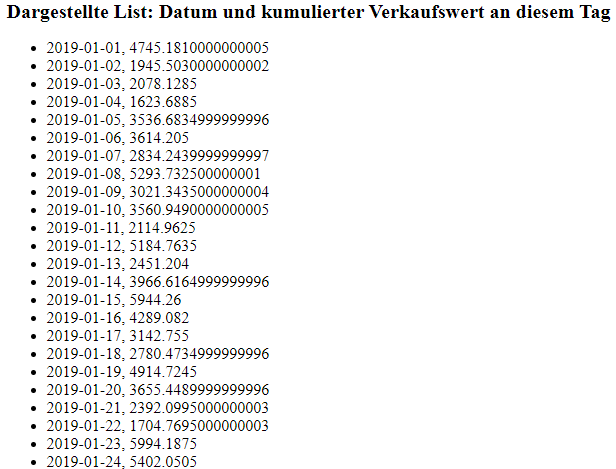
\includegraphics[width=10cm]{IMG/Zeitreihe}
		\caption{Ausschnitt der Zeitreihe mit zugehörigen Werten}
		\label{fig:Zeitreihe}
	\end{center}
\end{figure}

\noindent Die Expressivität profitiert von dieser besagten Liste, da wie vorher bereits beschrieben, das Verständnis dadurch verbessert wird und der Betrachter zu jedem Pixel den zugehörigen
Wert einsehen kann. Auch die Legende unterstützt die Pixelorientierte Darstellung in ihrem Ausdruck und trägt zur Verständigung der Aussagen bei, die diese Technik liefert. Ohne
die beiden vorher genannten Dinge, müssten bei der Expressivität Abstriche gemacht werden. Zudem wurden die Datenwerte in nur einer Zeile und nicht, wie für das Recursive
Pattern üblich, in mehrere Zeilen implementiert. DIes hat den eifnachen GRund der Lesbarkeit, da durch die beiden Filterebene die Länge der Stichprobe beliebig oft geändert werden
kann, sodass die Pixel immer wieder aus ihren festen Muster verrutschen würden und damit viel Aussagekraft dieser Visualisierung verloren gehen würde. \\

\begin{figure} [H]
	\begin{center}
		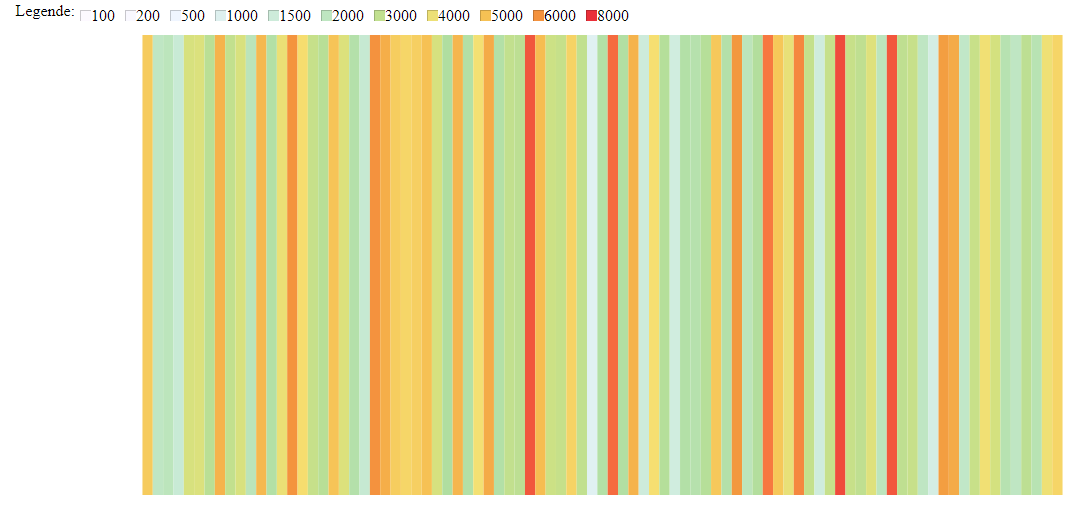
\includegraphics[width=10cm]{IMG/RecursivePattern.png}
		\caption{Visualisierung Drei - Pixelorientierte Darstellung}
		\label{fig:Zeitreihe}
	\end{center}
\end{figure}

\noindent Eine Alternative für die Pixelorientierte Darstellung gibt es nicht, da die Darstellung der Attribute auf Farbwerte nur eimalig vorhanden ist. Vielmehr könnte eine
Variation in der Anordnung der Pixel gefunden werden. So gibt es neben der Recursive Pattern Technik noch weitere Techniken, wie z.B. die Darstellung in Kreissegmenten oder
raumfüllende Kurven. \cite[5]{yeqiang2017visualizing} Allerdings sind diese Variationen für die Darstellung von Zeitreihen, wie sie in diesem Datensatz vorliegen, nicht besonders
gut geeignet, da z.b. die Darstellung in Kreissegmenten kein intuitives Lesen ermöglicht, weil Anfang und Ende der Zeitreihe nicht gut ersichtlich sind. Diese Alternativen würden
zu einer Abnahme bezüglich der Effektivität und Expressivität führen und wurden deswegen nicht benutzt.

\subsection{Interaktion}
Eine grundlegende Interaktionsmöglichkeit, die in diesem Projekt implementiert wurde, ist die Auswahl der Attribute durch Filter. Dieser Filter wurde in zwei Ebenen implementiert.
Die erste Ebene des Filter grenzt die Stichprobe hinsichtlich des gewählten Attributs ein. Durch die zweite Ebene des Filters kann die bereits eingegrenzte Stichprobe nochmals
nach einen ausgewählten Attribut gefiltert werden, sodass letztendlich eine Stichprobe, mit zwei festen Attributen daraus resultiert. Die erste Ebene des Filters wird direkt
unter dem Dropdown-Menü der Visualisierungstechniken angezeigt. Sie besteht aus den verschiedenen Dropdown-Menüs der verschiedenen Attribute und deren Ausprägungen. Die zweite
Ebene des Filters wird direkt unter der ersten Ebene angezeigt und enthält ebenfalls die Dropdown-Menüs der verschiedenen Attribute und deren Ausprägungen.\\

\begin{figure} [H]
	\begin{center}
		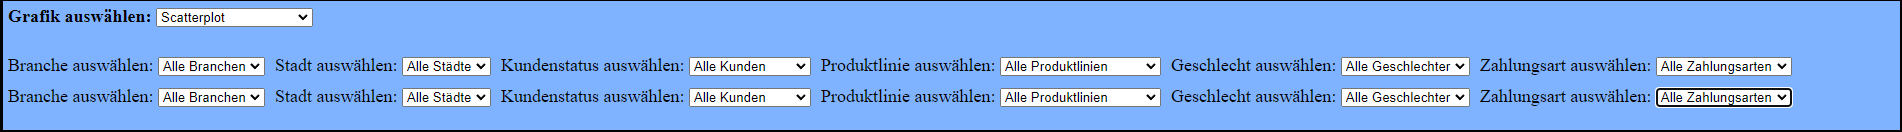
\includegraphics[width=16cm]{IMG/Filterung}
		\caption{Beide Ebenen der Filterung}
		\label{fig:Filterung}
	\end{center}
\end{figure}

\noindent Die gefilterte Stichprobe bleibt auch erhalten, wenn zwischen den Visualisierungstechniken gewechselt wird. So ist es möglich sich von einer gefilterten Stichprobe den
Scatterplot und im Nachgang auch noch die Pixelorientierte Darstellungen anzeigen zu lassen ohne die Filter wieder einzustellen. Dies garantiert einen flüßigen Vergleich
zwischen den Visualisierungstechniken.\\
Sinn der Implementierung dieser Filter ist auf der einen Seite eine übersichtliche Darstellung durch die Visualisierungstechniken zu gewährleisten,
andererseits können durch verschiedene Filterkombinationen viele neue Erkenntnisse bezüglich des Kunden- und Kaufverhalten erlangt werden. Mit einem einfachen Filter könnte
der Datensatz z.B. nur nach Geschlecht gefiltert werden, woduch zwar auch Erkenntnisse gewonnen werden, aber nicht reichlich. Mit der zusätzlichen Filter Ebene, ist es nun
möglich z.B. nach dem männlichen Geschlecht und Zahlungsart Kreditkarte zu filtern. \\
Zusätzlich zu den beiden Filter-Ebenen hätten die drei Visualisierungstechniken noch durch eine Farbauswahl miteinander verknüpft werden können. Hier wurde sich aber dagegen
entschieden, da noch weitere Entscheidungsparameter in Form von Buttons oder Dropdown-Menüs die Übersichtlichkeit des Programms verschlechtert hätten.\\
\noindent Innerhalb der Visualisierungstechniken gibt es ebenfalls Interaktionsmöglichkeiten. So wurde bei dem Scatterplot zwei Dropsdown-Menüs eingefügt, wo die Wahl der Achsen
festgelegt werden kann. Dieses Features ermöglicht die verschiedenen Variablen miteinander zu vergleichen und diese nach Zusammenhängen zu untersuchen.\\
Bei den Parallelen Koordinaten gibt es ebenfalls zwei Dropdown-Menüs, die für den Tausch zweier Achsen verantwortlich sind. Da von einer Achse immer nur die Zusammenhänge zu
ihren beiden benachtbaren Achsen angezeigt werden können, ist es daher wichtig die Reihenfolge der Achsen ändern zu können.

\section{Implementierung}
\subsection{Gesamtaufbau}
Das Projekt wurde grundsätzlich in fünf verschiedenen Modulen entwickelt. Darunter zählen Main.elm, Data.elm, Vis1.elm, Vis2.elm und Vis3.elm. Ergänzend zu diesen fünf Modulen
gibt es drei Hilfsmodule, die für die Datenvorverarbeitung oder für das Funktionieren bestimmter Funktionen notwendig sind. Hierunter zählen preparation.py, ein kleines
Python-Programm zur Umwandlung der Datum-Spalte in ein anderes Format. RecursivePattern.elm mit dem Zusatzmodul Helper.elm zählen ebenfalls zu den Hilfsmodulen, wobei diese beiden
Module von Alexander Kampf geschrieben wurden und lokal im Projektordner gespeichert werden mussten, da sie noch nicht in der offiziellen Elm-Bibliothek veröffentlicht wurden.

\begin{figure} [H]
	\begin{center}
		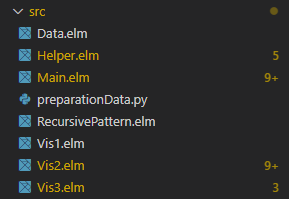
\includegraphics[width=7cm]{IMG/Modulgliederung}
		\caption{Gliedrung des Elm-Programms}
		\label{fig:Modulgliederung}
	\end{center}
\end{figure}

\noindent In Main.elm wurde standardmäßig die klassische Elm-Architektur bestehend aus Model, View und Update implementiert. Das Model enthält alle Parameter, die für die Auswahl der
Visualisierungen, der Achsen und der Attribute wichtig sind. Damit die Auswahl zwischen den gewählten Parametern auch klappt wurden viele verschiedene Msg definiert, welche dann
in der Update-Funktion aufgegriffen wurden und das Model mit den gewählten Parametern überschrieben haben. In der View-Funktion wurden alle sichtbaren Bestandteile, wie z.B.
Buttons, eingefügt sowie die fertigen Funktionen aus den anderen Modulen mit ihren Parametern aufgerufen. Zudem wurde hier der verwendete Datensatz mittels einer HTTP-Anfrage
eingeladen und in der init-Funktion neben all den anderen Parametern initialisiert. Diese eben beschriebenen Funktionalitäten machen das Modul Main.elm zum zentralen
Bestandteil des Programms.\\
In Data.elm wird alles behandelt was mit der Strukturierung und Verarbeitung der benötigten Daten zu tun hat.\\ Und in den drei Visualisierungs-Modulen
wird der Quellcode zur Darstellung der verschiedenen Visualisierungen implementiert. Die Implementierung der Visualisierungen wird später noch genauer beschrieben.\\
Zuvor müssen noch die für dieses Projekt erstellten Elm-Datenstrukturen behandelt werden. Im Zuge dieses Projekts wurde die Datenstruktur Sale erstellt. Diese besteht zum Teilen
aus Strings und Floats, jedoch auch aus Custom Types, die ebenfalls definiert werden mussten. Diese Custom Types wurden nur bei nominalen, endlichen Attributen des Datensatzes
eingeführt.

\begin{figure} [H]
	\begin{center}
		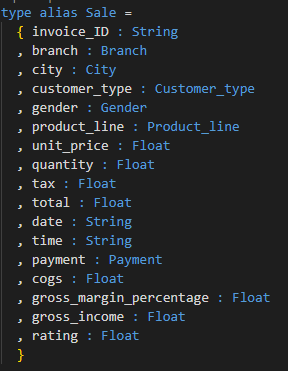
\includegraphics[width=5cm]{IMG/SaleDatenstruktur}
		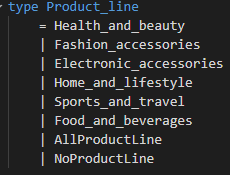
\includegraphics[width=5cm]{IMG/ProductLine}
		\caption{Sale Datenstruktur und Bsp. Custom Type}
		\label{fig:Sale}
	\end{center}
\end{figure}

\noindent Die Daten aus der eingeladenen csv-Datei wurden mittels Decodern in genau diese Datenstrukturen geschrieben, sodass am Ende der komplette Datensatz eine List von Sale
Objekten war. Innerhalb dieser Sale Objekte gab es dann bestimmt Attribute, wie z.B. der Kundenstatus, die als Custom Types fungierten und nur bestimmte Ausprägungen annehmen
konnten.\\ \\
\noindent In weiten Teilen sind bei der Implementierung keine Schwierigkeiten aufgetreten, einzig allein das überschreiben der csv-Daten in die jeweiligen Datenstrukturen
gestaltete sich zu Beginn etwas schwerer, da in dem Datensatz eine große Anzahl an nominalen DAten vorhanden war. Diese mussten dann alle in extra erstellte Datenstrukturen
geschrieben werden, was sich als sehr zeitaufwendig herausstellte. Zudem war die Verknüpfung der verschiedenen Msg mit der update-Funktion und der Buttons zu Beginn aufwendig.
Da die Buttons nur Strings akzeptierten musste zusätzlich für jeden erstellten Custom Type Funktionen geschrieben werden, die die Variants in Strings umwandeln und diese Strings auch
wieder zurück in die jeweiligen Variants der Custom Types.

\begin{figure} [H]
	\begin{center}
		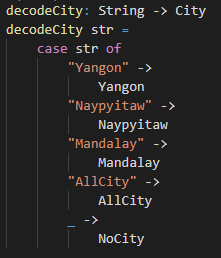
\includegraphics[width=4cm]{IMG/StrToCity}
		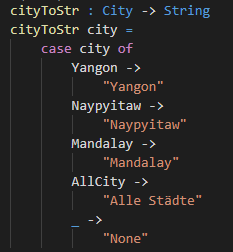
\includegraphics[width=4cm]{IMG/cityToStr}
		\caption{Beispiel für Umformungs-Funktion}
		\label{fig:Umformung}
	\end{center}
\end{figure}

\subsection{Implementierung Visualisierung 1}\label{Implementierung1}
Bei der Implementierung der ersten Visualisierung konnte ein Großteil des erstellten Quellcodes aus der Übung verwendet werden. Da in der Übung allerdings keine Filter zum
Einsatz kamen, musste bei dieser Implementierung zuvor die Funktion \textit{filterSalesData} geschrieben werden. Diese Funktion sorgt dafür, dass die Stichprobe, je nach
Belieben des Anwenders, nach bis zu zwei Attributen gefiltert werden kann. Anschließend werden von der gefilterten Stichprobe, die x- und y-Werte der gewünschten numerischen
Attribute in zwei Listen gespeichert, xFloat und yFloat. In diesen Listen von Tuples sind die Werte als Floats und die dazugehörigen Rechnungsnummern gespeichert. Danach
werden die beiden Listen durch \textit{List.map3} mit der Funktion \textit{toPoint} so verbunden, dass das Resultat eine Liste von Point Datenstrukturen ist. Diese Liste an
Points wurde dann abschließend in eine \textit{XYdatapoint} Datenstruktur geschrieben, sodass \textit{xyData} dann der scatterplot Funktion übergeben werden kann.

\begin{figure} [H]
	\begin{center}
		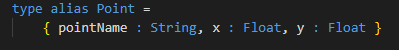
\includegraphics[width=6cm]{IMG/PointDatenstruktur}
		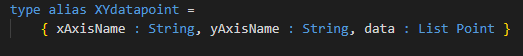
\includegraphics[width=7cm]{IMG/XYdatapoint}
		\caption{Point und XYdatapoint Datenstrukturen}
		\label{fig:Point_XYdatapoint}
	\end{center}
\end{figure}

\noindent Bei der Implementierung musste darauf geachtet werden, den Scatterplot so zu programmieren, dass die Interaktionsmöglichkeiten bestehen bleiben können.
So genügt es nicht, wie in den Übungen, die Auswahl der Achsen statisch an einem Punkt des Programms zu definieren, sondern es musste aus dem Model abgerufen werden. Da das
Model über Msg und die Interaktion mit den Buttons geändert werden kann, war somit die Interaktivität gegeben. Schwierigkeiten gab es bei der Implementierung dieser
Visualisierung keine.


\subsection{Implementierung Visualisierung 2}
Bei der Implementierung der parallelen Koordinaten konnte, genau wie bei dem Scatterplot, ein Teil des Quellcodes aus der Übung übernommen werden. Im Unterschied zur ersten
Visualisierung wurde hier nicht die XYdatapoint Datenstruktur verwendet, sondern die Datenstrukturen MultiDimPoint und MultiDimData verwendet. Erste besteht aus dem Namen als
String und einer Liste von Floats, die die Werte auf den jeweiligen Achsen darstellen sollen. MultiDimData dagegen beinhaltet eine Liste von Strings, die als Achsenbeschriftungen
dienen und als zweites eine Liste der MultiDimPoint Datenstruktur.
\begin{figure} [H]
	\begin{center}
		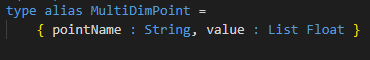
\includegraphics[width=8cm]{IMG/MultiDimPoint.png}
		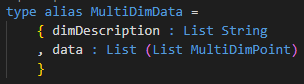
\includegraphics[width=6cm]{IMG/MulitDimData.png}
		\caption{MulitDimData und MultiDimPoint Datenstrukturen}
		\label{fig:Datenstrukturen_ParCoord}
	\end{center}
\end{figure}

\noindent Der eigentlichen parallelen Koordinaten werden in der Funktion \textit{parallelCoordinates} erstellt. Dazu werden zu Beginn Listen an Float Werten von jeden
numerischen Attribut erstellet und in mehreren Variablen gespeichert. Diese Listen werden dann genutzt, um die Werte der verschiedenen Achsen richtig skalieren zu können.
Anschließend wird dann über \textit{Shape.line} und \textit{Shape.linearCurve} die Punkte auf den verschiedenen Achsen miteinander verbunden, sodass erkennbar ist, welche Punkte
zu einer Datenreihen gehören. \\

\noindent Die Schwierigkeit hierbei war die Funktionalität des Achsentauschs zu implementieren. Dies wurde mithilfe von \textit{ListExtra.swapAt} gemacht. Diese Funktion sorgt dafür,
dass zwei Elemente einer Liste durch ihre Indexe getauscht werden können. Da die Achsenreihenfolge in einer Liste festgelegt wurde, konnte dies dadurch vollzogen werden. Damit
der Anwender entscheiden kann, welche Achse mit welcher anderen Achse getaucht wird, musste ein neuer Selector im Model implementiert werden. Dieser Selector in Form
eines Custom Types hat Variants für die verschiedenen Achsen. Nun mussten die verschiedenen Variants nur noch ihren entsprechenden Index von der Liste zugeordnet werden.
Dies geschah über die Funktion \textit{indexSelectorToInt}.

\noindent Die zwei Filterungsebenen sind hier ebenfalls anwendbar. Da \textit{filteredSalesData} und \textit{filteredSalesData2} einmal zu Beginn des view definiert wurden,
konnte diese Datenmenge auch in dieser Visualisierung wiederverwendet werden, was die Implementierung letztendlich vereinfachte.

\subsection{Implementierung Visualisierung 3}
Bei der Implementierung der Pixelorientierten Darstellung konnte ebenfalls auf dem Quellcode der Übungen aufgebaut werden. Allerdings wurde im Gegensatz zu der Übung hier nur
ein Level des Recursive Pattern Algorithmus angewendet. Grund dafür sind die zwei Filterebenen, denn diese können die Stichprobe auf unterschiedliche Arten und Weisen eingrenzen,
sodass immer unterschiedliche Längen der Stichprobe das Resultat sind. Aus diesem Grund ist es schwieriger die Datenwerte auf Pixel abzubilden, sodass es intuitiv von links nach
rechts lesbar bleibt. Dies stellte auch gleichzeitig eine Schwierigkeit bei der Implementierung dar, da an dieser Stelle viel experimentiert und probiert wurde, jedoch kein
zufriedenstellendes Ergebnis herauskam. Deswegen wurde sich letztendlich für die Darstellung in der Form entschieden, wie sie auch im finalen Programm vorzufinden ist.\\

\noindent Eine weitere Schwierigkeit stellte die Addition aller Gesamtausgaben an ihren jeweiligen Tagen dar. Die Idee war die Werte der Spalte Gesamtausgaben die auf den gleichen Tag fallen
zu addieren, um eine gute Übersicht zum Umsatz der Supermärlte an den jeweiligen Tagen zu geben. DAzu wurden zu erst alle Datumsangaben und alle Gesamtausgaben-Werte des Datensatzes
in zwei unterschiedliche Listen gespeichert. Anschließend wurden diese beiden Listen zu einer Liste von Tuples (\textit{tupleDateList}) verbunden und dem Datum nach sortiert
(\textit{(\textit{sortedTupleDateList})}). Nebenbei wurde noch eine Liste erstellt, wo jedes Datum nur einmal vorkommt und nicht, wie in der Tuple List, mehrmals
(\textit{uniqueDates}). Von der Liste \textit{uniqueDates} wurden durch List.map die Datumsangaben genommen und mit List.Extra.elemIndices die Indexe der Datumsangaben von der
Tuple Liste in einer neuen Liste \textit{indexList} gespeichert. Diese \textit{indexList} wurde dann schließlich dafür genutzt, um per List.Extra.getAt auf die Gesamtausgaben-Wert
der Tuple Liste zuzugreifen und diese ebenfalls in getrennten Listen je nach Datum in einer großen Liste zu speichern. Zum Schluss wurden dann die verschiedenen Listen innerhalb
der großen Liste durch List.sum addiert und das Resultat war am Ende eine Liste von Tuples, wo zu jedem Datum der dazugehörige kumulierte Gesamtausgaben-Wert stand
(\textit{dateSumList}). Diese Liste wurde dann für die Funktion \textit{recrusivePatternPlot} verwendet um die Werte auf die Pixel zu zeichnen. Die eben beschriebene Implementierung
war sehr zeitaufwendig sowie kompliziert und stellte damit die größte Schwierigkeit in dem gesamten Projekt dar.

\begin{figure} [H]
	\begin{center}
		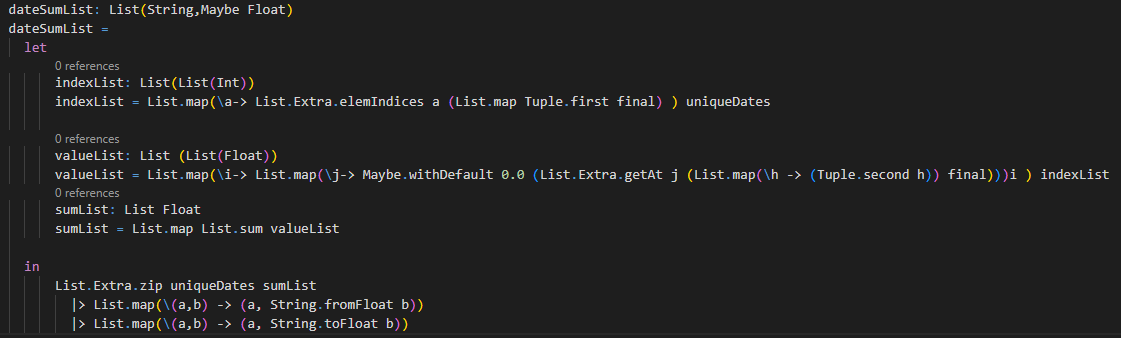
\includegraphics[width=17cm]{IMG/dateSumList}
		\caption{Code für Implementierung der Datumsangaben mit kumulierten Gesamtausgaben}
		\label{fig:Datum_Gesamtausgaben}
	\end{center}
\end{figure}

\subsection{Implementierung der Interaktion}
Die Implementierung der Interaktion wurde zum Teil schon im Abschnitt \ref{Implementierung1} beschrieben. Hierfür wurden die Funktionen \textit{filterSalesData} und
\textit{nominalAttrSelector} implementiert. Bei \textit{filterSalesData} wird durch den ersten Parameter geguckt, welches nominale Attribut ausgewählt wurde und durch den zweiten
Parameter, welche Ausprägung des zuvor gewählten nominalen Attributs ausgewählt wurde.

\begin{figure} [H]
	\begin{center}
		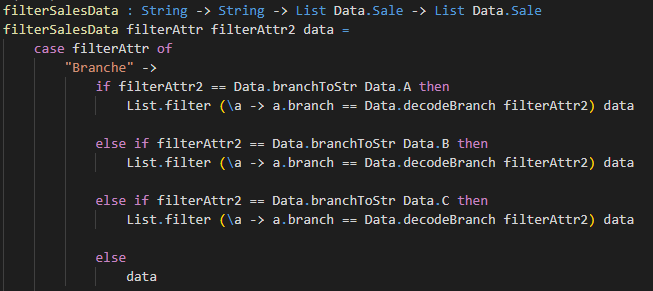
\includegraphics[width=14cm]{IMG/filterSalesData}
		\caption{Auszug von Funktion \textit{filterSalesData}}
		\label{fig:filterSalesData}
	\end{center}
\end{figure}

\noindent Die Funktion \textit{nominalAttrSelector} stellt sicher, dass der zweite Parameter von \textit{filterSalesData} in einen String umgewandelt wird, da nur Strings miteinander
auf Gleichheit überprüft werden können. Diese Funktion gibt es zudem noch in einer zweiten Variante für die zweite Filterebene.
\begin{figure} [H]
	\begin{center}
		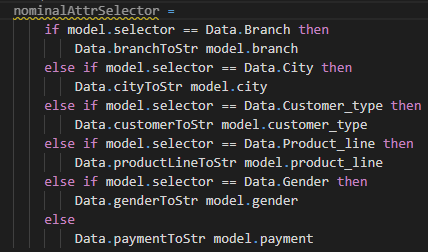
\includegraphics[width=12cm]{IMG/nominalAttrSelector}
		\caption{Funktion \textit{nominalAttrSelector}}
		\label{fig:filterSalesData}
	\end{center}
\end{figure}

\noindent Für die zweite Filterebene wurde zudem ein Selector2 im Model implementiert. Um die beiden Filterebenen nun anzuwenden, wurde zuerst die Funktion \textit{filterSalesData} mit
den gewählten Attributen über die Selector aufgerufen und in der Variable \textit{filteredSalesData} gespeichert. Diese Variable wurde dann wiederum nochmal in die Funktion
\textit{filterSalesData} eingefügt, diesmal jedoch mit \textit{Selector2} und \textit{nominalAttrSelector2}. Dies ermöglichte eine weitere Filterung der Daten, die bereits
einmal gefiltert waren.\\
\noindent Die Schwierigkeit hierbei war die Funktionen \textit{filterSalesData} und \textit{nominalAttrSelector} zu implementieren, da es zunächst etwas kompliziert war die
vielen Custom Types mit ihren Variants in Strings umzuwandeln und diese dann auf Gleichheit zu überprüfen. Allerdings wurde mit den genannten Funktionen alle Probleme behoben.

\section{Anwendungsfälle}
\subsection{Anwendung Visualisierung Eins: Scatterplot}
Wie bereits bei der Vorstellung des Scatterplots erwähnt, ist diese Visualisierungstechnik besonders wertvoll, um Zusammenhänge zwischen Variablen feststellen zu können. So kann
unteranderem festgestellt werden, inwiefern zwei numerische Attribute miteinander korrelieren und ob die Korrelation positiv oder negativ ist. Bei der Auswahl der Achsen auf
Gesamtausgaben als y-Achse und Bruttoeinkommen als x-Achse ist eine solche Korrelation festzustellen.
\begin{figure} [H]
	\begin{center}
		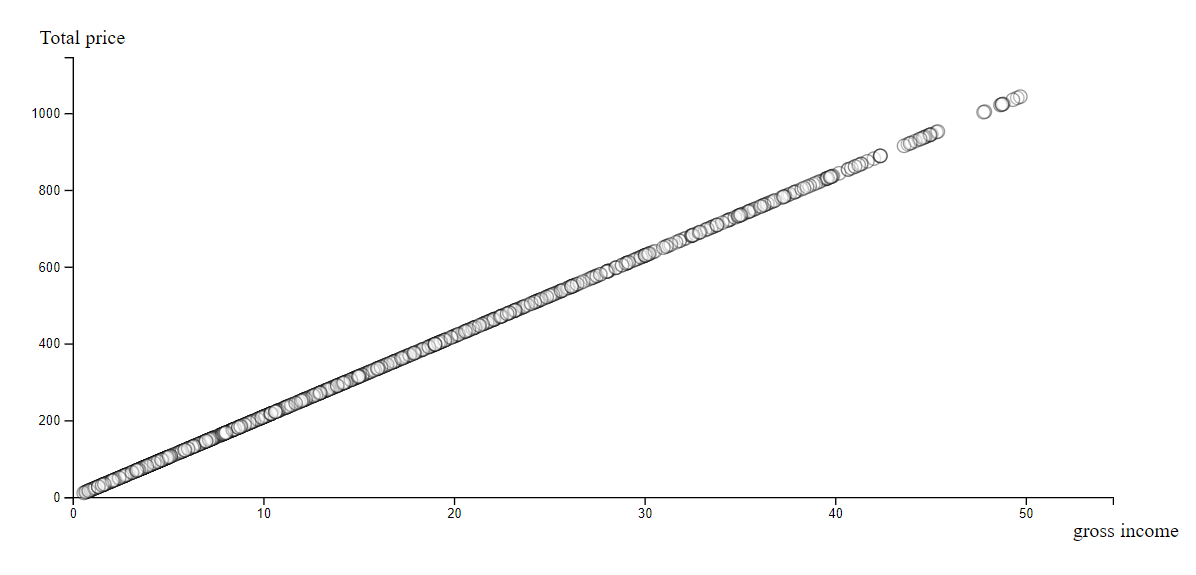
\includegraphics[width=15cm]{IMG/TotalPrice_GrossIncome.png}
		\caption{Zusammenhang Gesamtausgaben und Bruttoeinkommen}
		\label{fig:TotalPrice_Income}
	\end{center}
\end{figure}
\noindent Bei Betrachtung dieser Grafik fällt sehr schnell die linear steigende Gerade auf. Dieser stetig steigende lineare Verlauf steht für eine sehr starke und positive
Korrelation. Die Erklärung dafür ist, dass je höher das Bruttoeinkommen des Kunden ist, desto höher sind auch seine Ausgaben während eines Einkaufs im Supermarkt. Für die
Zielgruppen, also die Unternehmensführungen oder die Marketing-Abteilung des Supermarkts, ist dieser Anwendungsfall von besonderer Bedeutung, da sie ihr Angebot nun aufbauend
auf dieser Information anpassen können. Eine Möglichkeit wäre zum Beispiel, dass Produktangebot nach den Wünschen von Leuten mit einem hohen Bruttoeinkommen zu erweitern.
Eine andere Möglichkeit wäre die Einführung von Rabatten oder Vergünstigungen, sodass Menschen mit einem niedrigeren Bruttoeinkommen auch mehr kaufen. \\
\noindent Mit anderen Visualisierungstechniken wären diese Entdeckungen gar nicht oder nur sehr schwer rauszufinden gewesen. Bei der zuvor erwähnten Alternative für Scatterplots,
dem QQ-Plot, der auf die Verteilungen beider Variablen vergleicht, wäre ein solcher Zusammenhang nicht zu erkennen gewesen.

\subsection{Anwendung Visualisierung Zwei: Parallele Koordinaten}
Die Parallelen Koordinaten erweitern die Funktionalität des Scatterplots in dem sie zusätzliche Dimensionen betrachtbar machen und somit mehr als zwei Variablen auf Zusammenhänge
überprüft werden können.

\begin{figure} [H]
	\begin{center}
		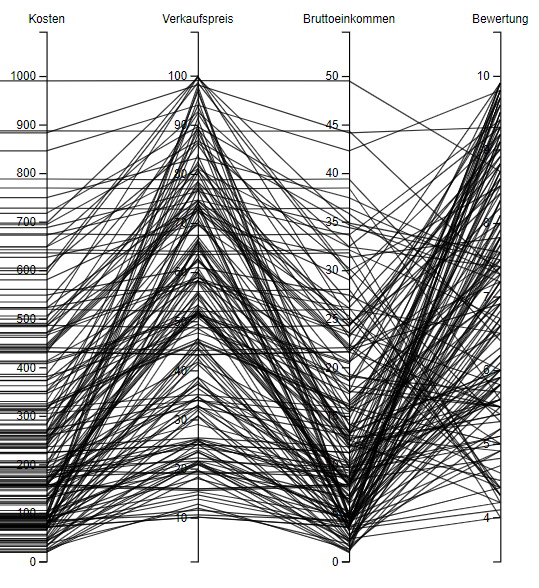
\includegraphics[height=9cm]{IMG/ZusammenhangParCoord.png}
		\caption{Ausschnitt von Parallelen Koordinaten mit Daten aus Stadt: Yangon und Geschlecht: Mann}
		\label{fig:ZusammenhangParCoord}
	\end{center}
\end{figure}

\noindent Bei diesem Ausschnitt der Parallelen Koordinaten von den vier Achsen: Kosten, Verkaufspreis, Bruttoeinkommen und Bewertung sind leichte Zusammenhänge zwischen den
einzelnen Variablen zu erkennen. So kaufen Personen mit einem niedrigeren Bruttoeinkommen verhältnismäßig oft kostenintensive Güter ein. Hier besteht also eine negative
Korrelation. Grund dafür könnten z.B. teure, lebensnotwendige Güter sein, die gekauft werden müssen.
Zusätzlich dazu ist erkennbar, dass die selben Personen ihren Einkauf mit einer hohen Punktzahl bewerten, was auf eine hohe Kundenzufriedenheit schließen lässt. Diese Information
ist ebenfalls sehr wichtig für die Zielgruppen. Hierbei sollte der Unternehmensführung klar werden, dass Leute mit einem niedrigen Einkommen sehr zufrieden mit dem Einkauf und
dem Service der Supermärkte sind. Dementsprechend sollte das Vertrauen und die Treue dieser Kunden nicht ausgenutzt werden und sie stattdessen stärker gefördert und unterstützt
werden.\\
\noindent Als Alternative zu Parallelen Koordinaten wurden im Abschnitt \ref{Visualisierung2} die Darstellung mittels Icons genannt. Dieses eben beschriebene Muster hätte dort
auch gefunden werden können, jedoch mit einem größeren Aufwand. Da alle Dimensionen auf dem selben Icon abgebildet werden müssen, sind Zusammenänge dort sehr schwerer zu erkennen.
Eine Lösung dafür wäre, dass nur bestimmte Dimensionen auf den Icons abgebildet werden, was aber wiederrum mit einer Minderung der Effektivität und Expressivität einhergeht.

\subsection{Anwendung Visualisierung Drei: Pixelorientierte Darstellung}
Die Pixelorientierte Darstellung wurde zum Erkennen von Ausreißern und der Abbildung der Werte auf Farbe implementiert. Hohe Werte wurden, wie bereits vorher im Bericht
beschrieben, auf warmen Farben und niedrige Werte auf klate Farben abgebildet.

\begin{figure} [H]
	\begin{center}
		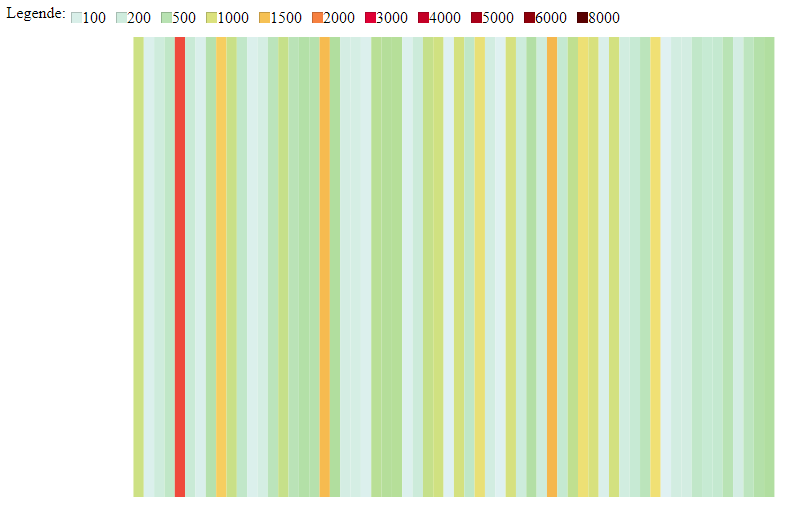
\includegraphics[height=9cm]{IMG/PixelFoodFrau.png}
		\caption{Pixelorientierte Darstellung mit Daten aus Produktlinie: Food and beverages und Geschlecht: Frau}
		\label{fig:PixelFoodFrau}
	\end{center}
\end{figure}

\noindent Bei dieser Grafik sieht man sehr schön einen klaren Ausreißer zu Beginn der Zeitreihe. Dieser fällt durch die auffallend rote Farbe sofort ins Auge.
Wenn nun auf die unter der Visualisierung abgebildete Liste mit den Datumsangaben und ihren zugehörigen kumulierten Gesamtausgaben guckt, sieht man den Wert 2396.457 und
das als Datum 2019-01-08. Jetzt kann man in Erfahrung bringen, ob an diesem Tag bestimmte Ereignisse stattgefunden haben und ob diese Ereignisse in Zukunft wieder auftreten.
Unabhängig davon wissen die Zielgruppen nun trotzdem, dass am 8. Januar 2019 Frauen besonders viel Essen und Getränke gekauft haben. Diese Information kann die Unternehmensführung
nun benutzen, um sich, falls dieses Muster sich wiederholt, auf solche Steigerungen der Nachfrage vorzubereiten.\\
\noindent Wie bereits im Abschnitt \ref{Visualisierung3} angedeutet, gibt es keine wirklichen Alternativen zu der Pixelorientierten Darstellung. Aus diesem Grund wäre die
Information, die hier gewonnen wurde auch nicht durch eine andere Visualisierung reproduzierbar gewesen.

\section{Verwandte Artikel}
Nach einer kurzen Literaturrecherche wurden folgende zwei Artikel verwendet:\\

\noindent Bei dem ersten Artikel handelt es sich um \textit{Using data visualization for supermarket retail analysis} von Shuming Wang und Phisanu Chiawkhun. \cite{wang2022data}
Zu Beginn gehen die beiden Autoren, genau wie in diesem Bericht, auf die Gründe für eine Analyse von Kunden- und Geschäftsdaten ein. Hierbei heben sie hervor, dass es äußerst
wichtig für Supermärkte ist, den Wert verschiedener Kundengruppen zu kennen. Darauf aufbauend lässt sich laut Wang und Chiawkhun dann eine sehr spezifische Marketingkampagne
starten, die kaufbereite sowie loyale Kunden ansprechen und überzeugen soll. Diese Vorgehensweise stellt einen Unterschied zu den Untersuchungsvorgängen in diesem Bericht dar,
da hier aufgrund unausreichender Daten nicht der Wert von verschiedenen Kundengruppen bestimmt werden konnte.\\
Allerdings behandelt der Bericht von Wang und Chiawkhun die gleichen Problemstellungen und spricht die gleichen Zielgruppen, wie dieser Bericht an. So wurde in beiden Berichten
die stetig wachsende Konkurrenz im Einzelhandel als größtes Problem identifiziert. Die Bedeutung der Ausrichtung des Angebots nach Kundenwünschen wurde ebenfalls von beiden
unterstrichen. Zusätzlich sprechen beide Bericht mit ihren Analyseergebnissen die Unternehmensführungen der Supermärkte sowie die Marketing-Abteilungen an.\\
Im weiteren Verlauf der Untersuchung kam es vermehrt zu Abweichungen in der Vorgehensweise beider Berichte. So führten Wang und Chiawkhun ihre Analysen explizit für
jedes Jahr einzeln durch. Dadruch konnten genau Angaben zur Entwicklung vom Kaufverhalten der Kunden gemacht werden. Dies wurde in diesem Bericht nicht gemacht, da der
verwendete Datensatz nur Daten beinhaltete, die in einem Zeitraum von drei Monaten stattfanden.\\
Visualisiert wurden die Daten durch Line Graphs, Farbdarstellung in Tabellenform, Balkendiagrammen und Kreissegmentdiagrammen. Diese Darstellungsformen wurden im Zuge dieses
Berichts ebenfalls nicht verwendet, da dieser Bericht mehr auf die Zusammenhänge und Abhänigkeiten zwischen einzelnen Parametern des Datensatzes fokussiert war, als Verteilungen
oder Häufigkeitsverteilungen von bestimmten Variablen einzeln zu betrachten.\\
Zusammenfassen kann gesagt werden, dass beide Berichte in ihrem Fundament viele Ähnlichkeiten aufweisen, sich in der Art und Weise der Untersuchungsvorgänge jedoch voneinander
unterscheiden.\\
\noindent Bei dem zweiten Artikel handelt es sich um \textit{Data visualization: an exploratory study into the software tools used by businesses}.\cite{diamond2017data}
In diesem Bericht von Diamond und Mattia geht es vorallem um die stetig wachsende Bedeutung der Datenvisualisierung in der heutigen Zeit. Diese These unterstreichen die Autoren
mit einer Grafik, wo die Anzahl von erforderlichen Statistiksoftware-Kenntnissen je nach Jobbörse eingetragen wurden. Des Weiteren vollzogen die beiden Autoren, dann ebenfalls
eine Datenvisualisierung bezüglich Verkaufsdaten mit verschiedenen Visualisierungstootls. Hierbei benutzen sie unteranderem Microsoft Excel, Power BI, Tableau und
Watson Analytics. Als Visualisierungstechniken wurden vorallem Balkendiagramme, Line Graphs und Kreissegmentdiagramme verwendet. Diese Visualisierungstechniken wurden im Zuge
dieses Berichts nicht verwendet, da wie bereits zum ersten Artikel beschrieben, hier eher der Zusammenhang zwischen den einzelnen Attributen des Datensatzes untersucht wurde.\\
Bei der Analyse der Daten wurde sich vermehrt auf die geographischen Unterschiede bei dem Datensatz fokussiert. So wurden Verkaufsdaten aus den Ländern USA, Deutschland,
Frankreich, Australien und dem Vereinigten Königreich ausgewertet. In diesem Bericht wurde auch eine geographische Unterscheidung gemacht, jedoch nicht zwischen Ländern,
sondern zwischen den Städten Yangon, Naypyitaw und Mandalay.
\\ In ihrer Zusammenfassung schrieben Diamond und Mattia, dass die Anwendung von sogenannten Daten-Dashboards immer wichtiger wird und dass Universitäten und Schulen, ihre Schüler
auf die Anwendnung von Visualisierungstools vorbereiten sollten. Eine ähnliche Schlussfolgerung wird in diesem Bericht auch gefällt. Die wachsende Konkurrenz und der stetig steigende
Wettbewersdruck nimmt die Unternehmen von Supermärkten in die Pflicht ebenfalls verstärkt auf die Analyse und Visualisierung ihrer eigenen Daten zu setzen. Demzufolge brauchen
sie auch Datenanalysten, die diese Aanalysen und Visualisierungen druchführen und die aus diesem Grund von den Unternehmen auch gefördert werden sollten.\\
Zusammenfassend kann gesagt werden, dass die Problemstellungen der beiden Berichte etwas unterschiedlich waren, die Schlussfolgerungen jedoch mehrere Parallelen ausweisen.  



\printbibliography


\end{document}